\documentclass[twocolumn]{jsarticle} %articleではなくjsarticleにすることで、「参考文献」と日本語で出る.
%\usepackage{graphicx} % Required for inserting images
\usepackage{amsfonts}
\usepackage{amsmath}
\usepackage{amssymb, amsfonts, latexsym, mathtools}
%これ3つセットで正しくpngが表示される!
\usepackage[dvipdfmx]{graphicx}
\usepackage[dvipdfmx]{color}
\usepackage[dvipdfmx]{geometry}

\usepackage{enumitem}
\usepackage{titlesec}
\usepackage{caption}
\usepackage{setspace}
\usepackage{here}
\usepackage{physics}
\usepackage{bm}
\usepackage{url} %urlをじか張りできる。
\usepackage{subfigure} %ずを横並びにする。
\usepackage{booktabs}
\usepackage{array}
\usepackage{color}
%\usepackage{tikz}
%\usepackage{tikz-timing}[2009/05/15]

\renewcommand{\labelenumi}{(\arabic{enumi})}


\title{物理学実験II 顕微鏡光学系}
\author{05251559 菱伊勇介}
\date{実験日: 2025年12月11, 15 ,17日共同実験者: NaN \\レポート提出日: \today}

\begin{document}
\maketitle

\section*{実験1. レンズの公式(単レンズ、複合レンズ)}
\subsection*{目的}
単レンズの公式
\begin{equation}
\dfrac{1}{a}+\dfrac{1}{b}=\dfrac{1}{f} \label{eq:lens_formula}
\end{equation}
が本当に成り立つかを確認する。
また、複数のレンズを組み合わせた場合に適用される合成焦点距離の概念を検証し、
密着配置・間隔あり配置の違いが結像位置にどのように影響するかを調べる。

さらに、実験ではレンズホルダー内のレンズの主点位置を厳密に特定することが困難であるという
現実的な制約を踏まえ、ニュートンの結像式など主点位置を必要としない測定手法をどのように実験的に確立できるかを検討する。この過程を通じて、光学設計における結像条件と測定手法の基礎を習得することを目的とする。
\\

\subsection*{方法}
光源として白色LEDを用い、光源、レンズ、スクリーンを光学レール上に一直線に配置した。
単レンズとして焦点距離 $f=200\,\mathrm{mm}$ のレンズを用い、
光源とレンズの距離 $L_1$ を固定した上で、
スクリーンを前後に移動させ、像が最も鮮明に結像する位置を探索した。
このときのレンズとスクリーンの距離 $L_2$ を測定した。

次に複合レンズ系として、焦点距離 $f_1=200\,\mathrm{mm}$、
$f_2=500\,\mathrm{mm}$ の2枚のレンズを用いた。
光源、レンズ1、レンズ2、スクリーンを順に配置し、
スクリーンを移動させて結像位置を求めた。
レンズ間隔を変化させた場合および2枚のレンズを密着させた場合について、
それぞれ同様の測定を行った。

なお、複合レンズの理論値を計算する際には、図\ref{fig:compound_lens}の式
\begin{equation}
  \frac{1}{f}=\frac{1}{L_1+\delta_1}+\frac{1}{L_2+\delta_2} \label{eq:compound_lens}
\end{equation}
を用いた。

\begin{figure}[H]
  \centering
  \includegraphics[width=0.95\linewidth]{./figure/1_gosei_eq.png}
  \caption{複合レンズ系と使った公式。実験当日配布資料から引用。}
  \label{fig:compound_lens}
\end{figure}

\clearpage
\onecolumn
\subsection*{結果}
単レンズの系の結果を表\ref{tab:single_lens}に、複合レンズの系の結果を表\ref{tab:compound_sep}に示す。
\begin{table}[H]
\centering
\caption{単レンズ($f=200\,\mathrm{mm}$)における結像位置の測定結果}
\label{tab:single_lens}
\begin{tabular}{ccc}
\toprule
$L_1$ [mm] & 実測 $L_2$ [mm] & 理論値 $L_2$ [mm] \\
\midrule
400 & $400\pm 1$ & 400 \\
300 &  $600 \pm 1$& 600 \\
600 &  $300 \pm 1$& 300 \\
\bottomrule
\end{tabular}
\end{table}

\begin{table}[H]
\centering
\caption{複合レンズ系($f_1=200\,\mathrm{mm}$,$f_2=500\,\mathrm{mm}$)における結像位置}
\label{tab:compound_sep}
\begin{tabular}{cccc}
\toprule
レンズ間隔$d$ [mm] & $L_1$ [mm] & 実測 $L_2$ [mm] & 理論値 $L_2$ [mm] \\
\midrule
25 (\text{密着\footnotemark})& 400& $215\pm3$ & 214.3\\
100 & 400 & $188 \pm 3$ & 187.5  \\
200 & 400 & $746 \pm 3$ & 142.9 \\
\bottomrule
\end{tabular}
\end{table}
\footnotetext{レール上でレンズを密着させても、実際にはレンズを固定するホルダーを密着させただけで、レンズの中心間では25mmの隙間が存在した。}

\twocolumn
\clearpage
\subsection*{考察}
\subsection*{レポートのための課題1}
\begin{enumerate}
  \item 単レンズ、複合レンズともに、測定誤差の範囲で一致した。
  すなわち、本実験の結果はレンズの公式(\ref{eq:lens_formula})および複合レンズの公式(\ref{eq:compound_lens})を支持するものであった。
  \item 以下のようなステップを遂行すると良い。記号は図\ref{fig:newton_setup}に揃えた。
  \begin{enumerate}
  \item \textbf{平行に光を入射する。}\\
  レンズ群に平行光を入れて、スクリーン上で1点に集中する位置を探す。  
  このときの位置を後側焦点面$F'$とみなし、その面の位置をレール上で記録する。

  \item \textbf{後側焦点面からの距離 $t'$ を基準に、像位置を測る。}\\
  光源(または物体)を前方近距離に置き、スクリーンを$F'$からより遠ざけることで結像する位置$P'$を記録する。  
  「像面」と「後側焦点面」の間隔$F'P'$を $t'$として測定する。
  \begin{figure}[H]
    \centering
    \includegraphics[width=0.8\linewidth]{./figure/1_newton_setup.png}
    \caption{ニュートンの式を用いた測定の概念図。実験当日配布資料から引用。}
    \label{fig:newton_setup}
  \end{figure}

  \item \textbf{前側焦点面からの距離 $t$ を測る。}\\
  レンズ系を反転して、再び平行光を入れ、物体位置と「前側焦点面」の距離 $t$ を(a)(b)と同様の手順で測定する。  
  (反転が難しい場合は、同一レンズ系の前後を入れ替えて同等操作を行えば良い。)

  \item \textbf{ニュートンの式を用いて、焦点距離 $f$ を求める。}\\
  前側焦点面から物体までの距離 $t$、
  後側焦点面から像までの距離 $t'$ に対して、
  ニュートンの式
  \[
    tt' = f^2
  \]
  を用いる。ここで、$f=f'$を仮定した。
  物体位置を変えて複数組の $(t, t')$ を測定し、
  $tt'$ が一定となることを確認することで、
  主点位置を用いることなく焦点距離 $f$ を決定する。
\end{enumerate}
このようにして、物点距離$t+f$と、像点距離$t'+f$とを主点位置$H,H'$を特定せずに測定できる。
\end{enumerate}

\clearpage

\section*{実験2.集光の回折限界}
\subsection*{\underline{目的}}
レーザー光を集光する実験を通して、開口を絞っても集光点はある大きさ以下には小さくならず、
光の集光には回折に起因する限界があることを確認する。

\subsection*{\underline{方法}}

図\ref{fig:exp2_setup}に示す作図に基づき、レーザー光(スポット径 $\phi=2.9\,\mathrm{mm}$)を拡大するため、
焦点距離 $f=-50\,\mathrm{mm}$ および $f=750\,\mathrm{mm}$ のレンズを用いたアフォーカル光学系を構成した。  
拡大後のレーザー光のスポット径を測定するとともに、スクリーンを前後に移動させることで、出射光が平行光であることを確認した。

\begin{figure}[H]
  \centering
  \includegraphics[width=0.95\linewidth]{./figure/2_setup.png}
  \caption{レーザー光拡大のために作図したアフォーカル光学系。
焦点距離 $f=-50\,\mathrm{mm}$ の凹レンズと $f=750\,\mathrm{mm}$ の凸レンズを用い、
平行光が再び平行光として出射する配置を作図により決定した。倍率は15倍である。}
  \label{fig:exp2_setup}
  
\end{figure}

次に、拡大後のレーザー光の光路上に絞りを設置し、
絞りを閉じるとスクリーン上のスポット径が小さくなることを確認した。

その後、スクリーンの代わりに焦点距離 $f=500\,\mathrm{mm}$ のレンズを配置し、
その焦点面にスクリーンおよびカメラを設置して集光像を観察した。減光フィルタを用いて光量を調整した後、カメラを前後に移動させ、集光スポットが最も小さくなる位置に合わせた。

絞りの開口径を段階的に変化させながら集光スポット像を取得し、
各条件における輝度分布を解析した。集光スポットの縁を直接定義することが困難であるため、
輝度分布を二次元ガウス分布でフィッティングし、その半値半幅を集光スポット半径 $r$ の指標として用いた。
なお、カメラの素子間隔は $5.2\,\mu\mathrm{m}$ である。

\clearpage
\onecolumn
\subsection*{\underline{結果}}

アフォーカル光学系により拡大したレーザー光のスポット径は \underline{$\phi = 45 \pm 3\,\mathrm{mm}$} であり、
スクリーン位置を変えてもほぼ一定であることから、出射光が平行光であることを確認した。

次に、焦点距離 $f=500\,\mathrm{mm}$ のレンズを用いて集光を行い、
絞りの開口直径 $D$ を変化させて集光スポット像を取得した。
ガウスフィッティングにより求めたスポット半径 $r$ を
$1/D$ に対してプロットした結果を図\ref{fig:exp2_result}に示す。

図より、開口直径 $D$ を小さくするほどスポット半径 $r$ は単調に増加し、
$r$ は概ね $1/D$ に比例する振る舞いを示した。

\begin{figure}[H]
  \centering
  \includegraphics[width=0.75\linewidth]{./figure/2_result.png}
  \caption{集光スポット半径 $d$ と開口直径 $D(=2a)$ の関係。横軸は $1/D$ とし、測定値(点)と回折限界の理論式 $d_{\mathrm{th}}=1.22\lambda f/D$(実線)を比較した。}
  \label{fig:exp2_result}
\end{figure}


\twocolumn
\subsection*{\underline{考察}}

\subsection*{レポートのための課題2}

幾何光学的には、レンズ3に平行光を入射し、カメラをその焦点面に置いた場合、
集光像は幾何学的な一点になると考えられる。
しかし実際には、円形開口を通過した光は回折の影響を受け、
焦点面では有限の大きさを持つ円盤状の像を形成する。

円形開口による回折の理論によれば、集光スポットの大きさは
開口直径 $D$ に反比例し、
\[
r = 1.22\,\frac{\lambda f}{D}
\]
で与えられることが知られている\footnote{これはエアリーディスクの最小の暗環の半径を与える式だ。}。
本実験では、ガウスフィッティングによって得られた半値半幅を
集光スポット半径 $r$ の指標として用いたため、
理論式で定義されるエアリーディスクの半径とは定義が異なり、
数値としては定数倍のずれが生じていると考えられる。

一方で、測定結果を $1/D$ に対して整理すると、
開口直径 $D$ を小さくするほどスポット半径 $r$ が増加し、
$r$ が $1/D$ に比例するという理論的予想に沿う振る舞いが確認された(図\ref{fig:exp2_result})。
以上より、本実験により、集光像の大きさが回折によって制限されること、
すなわち集光には回折限界が存在することを実験的に確認できた。

\clearpage

\section*{実験3. クリティカル照明}
\subsection*{\underline{目的}}
クリティカル照明は、光源の像を試料面(観察面)に直接結像させることで高い照明強度を得る照明法であるが、
光源の輝度分布や発光素子の構造がそのまま試料面に投影され、照明ムラを生じやすいという欠点を持つ。
本実験では、LED光源とレンズ($f=200\,\mathrm{mm}$)からなる簡単な照明光学系を組み、
スクリーン位置を変化させることで、(i)光源像がスクリーン上に結像して最も明るいが一様でない状態(クリティカル照明)と、
(ii)光源像がぼけて一様になるが暗い状態とを観察し、
その違いを確認する。さらに、スクリーン中央付近を可能な限り明るく、
かつ一様に照明するための光源とレンズの配置条件を検討し、幾何光学に基づいて両照明法の特徴を整理することを目的とする。

\subsection*{\underline{方法}}
光源として白色LEDを用い、LED光源、レンズ、スクリーンを光学レール上に一直線に配置した。
レンズには焦点距離 $f=200\,\mathrm{mm}$ の凸レンズを用いた。

まず、スクリーン位置を変化させながら、光源像がスクリーン上に明瞭に観察される条件を探索した。
スクリーン上に発光素子のパターンが結像する配置では、照明は非常に明るいが空間的なムラを伴うことを確認し、
これをクリティカル照明の条件として記録した。

次に、一様照明の条件として、光源をレンズの前側焦点位置に配置し、光源とレンズの距離を $f$ に一致させた。
すなわち光源からレンズまでの距離を $200\,\mathrm{mm}$ に設定した。
このとき、レンズ通過後の光はほぼ平行光となり、スクリーン上には光源像が形成されず、比較的一様な照明が得られた。
スクリーンを前後に移動させ、照明の一様性および光線の半径がほとんど変わらないことを確認した。

\subsection*{\underline{結果}}
クリティカル照明の条件(光源像がスクリーン上に結像する配置)では、スクリーン上に光源(発光素子)の構造が明瞭に観察された。
このとき照明強度は大きい一方で、光源の輝度分布がそのまま投影されるため空間的なムラが顕著であった(図\ref{fig:critical_illumination})。

一方、光源をレンズの前側焦点位置に配置し、光源とレンズの距離を $f=200\,\mathrm{mm}$ に一致させた場合、レンズ通過後の光はほぼ平行光となり、スクリーン上に光源像は形成されなかった。
この配置では照明は比較的一様になったが、光が広い領域に分散するため、クリティカル照明と比べて明るさは低下した(図\ref{fig:uniform_illumination})。

\begin{figure}[H]
  \centering
  \includegraphics[width=0.95\linewidth]{./figure/3_critical-01.png}
  \caption{クリティカル照明の概念図。光源の像が観察面に結像するため、光源の構造がそのまま投影され、明るいが照明ムラが生じる。}
  \label{fig:critical_illumination}
\end{figure}

\begin{figure}[H]
  \centering
  \includegraphics[width=0.95\linewidth]{./figure/3_critical-02.png}
  \caption{一様照明(光源をレンズの焦点に配置)の概念図。レンズ通過後の光が平行光となり、観察面に光源像が結像しないため、一様な照明が得られる。}
  \label{fig:uniform_illumination}
\end{figure}

\subsection*{\underline{考察}}
\subsection*{レポートのための課題3}
図\ref{fig:critical_illumination}のように、クリティカル照明では、光源の像がスクリーンに結像するように光学系が構成される。
したがって、光源の輝度分布や発光素子の構造がそのまま観察面に投影され、照明は明るい一方で空間的なムラを生じやすい。
これは、観察面上の各点が光源内の対応する点と1対1に対応するためである。

一方、図\ref{fig:uniform_illumination}のように、光源をレンズの前側焦点に置くと、レンズ通過後の光はほぼ平行光となり、観察面上に光源像は結像しない。
このとき観察面上の各点には光源の広い領域からの光が重なって到達するため、光源の構造は平均化され、照明は比較的一様となる。
ただし光は広い範囲に分散するため、単位面積あたりの照明強度は低下する。

以上より、クリティカル照明は高い照明強度を得られる代わりに一様性に劣り、一様照明は一様性を得られる代わりに明るさが低下するというトレードオフの関係にあることが分かる。

\clearpage



\section*{実験4. ケーラー照明}
\subsection*{\underline{目的}}
ケーラー照明は、視野面における照明の一様性と、開口数に対応する角度分布の制御とを独立に実現する照明法である。
本実験では、集光レンズおよびコンデンサレンズを用いてケーラー照明系を構成し、
(i)光源像が開口絞り面に結像し、(ii)視野絞りが試料面に結像することを確認する。
さらに、視野絞りおよび開口絞りを調整して、視野の明るさ・一様性およびコントラストがどのように変化するかを観察し、
クリティカル照明との違いを理解することを目的とする。

\subsection*{\underline{方法}}
図\ref{fig:kohler_setup}および図\ref{fig:kohler_sakuzu}に示すように、光源、集光レンズ、視野絞り、開口絞り、コンデンサレンズ、試料を光学レール上に順に配置し、
ケーラー照明系を構成した。
集光レンズおよびコンデンサレンズには焦点距離 $f=200\,\mathrm{mm}$ の凸レンズを用いた。
図の配置(集光レンズ位置 400\,mm、視野絞り位置 600\,mm、開口絞り位置 800\,mm、コンデンサレンズ位置 1000\,mm、
試料位置 1400\,mm)を初期値として光学系を組んだ。

まず、視野絞りの像が試料面に結像するようにコンデンサレンズおよび試料位置を調整し、視野を規定できることを確認した。
次に、光源像が開口絞り面に結像するように集光レンズおよび開口絞り位置を調整し、開口絞りの開閉によって試料面の照明の角度分布(NA)が変化することを確認した。
最後に、視野絞りおよび開口絞りをそれぞれ段階的に変化させ、視野の明るさ・一様性および像コントラストの変化を観察した。

\begin{figure}[H]
  \centering
  \includegraphics[width=0.95\linewidth]{./figure/4_kohler.png}
  \caption{ケーラー照明の光学系。視野絞りは試料面に結像し、開口絞り面には光源像が結像する。図は実験テキストから引用。}
  \label{fig:kohler_setup}
\end{figure}

\begin{figure}[H]
  \centering
  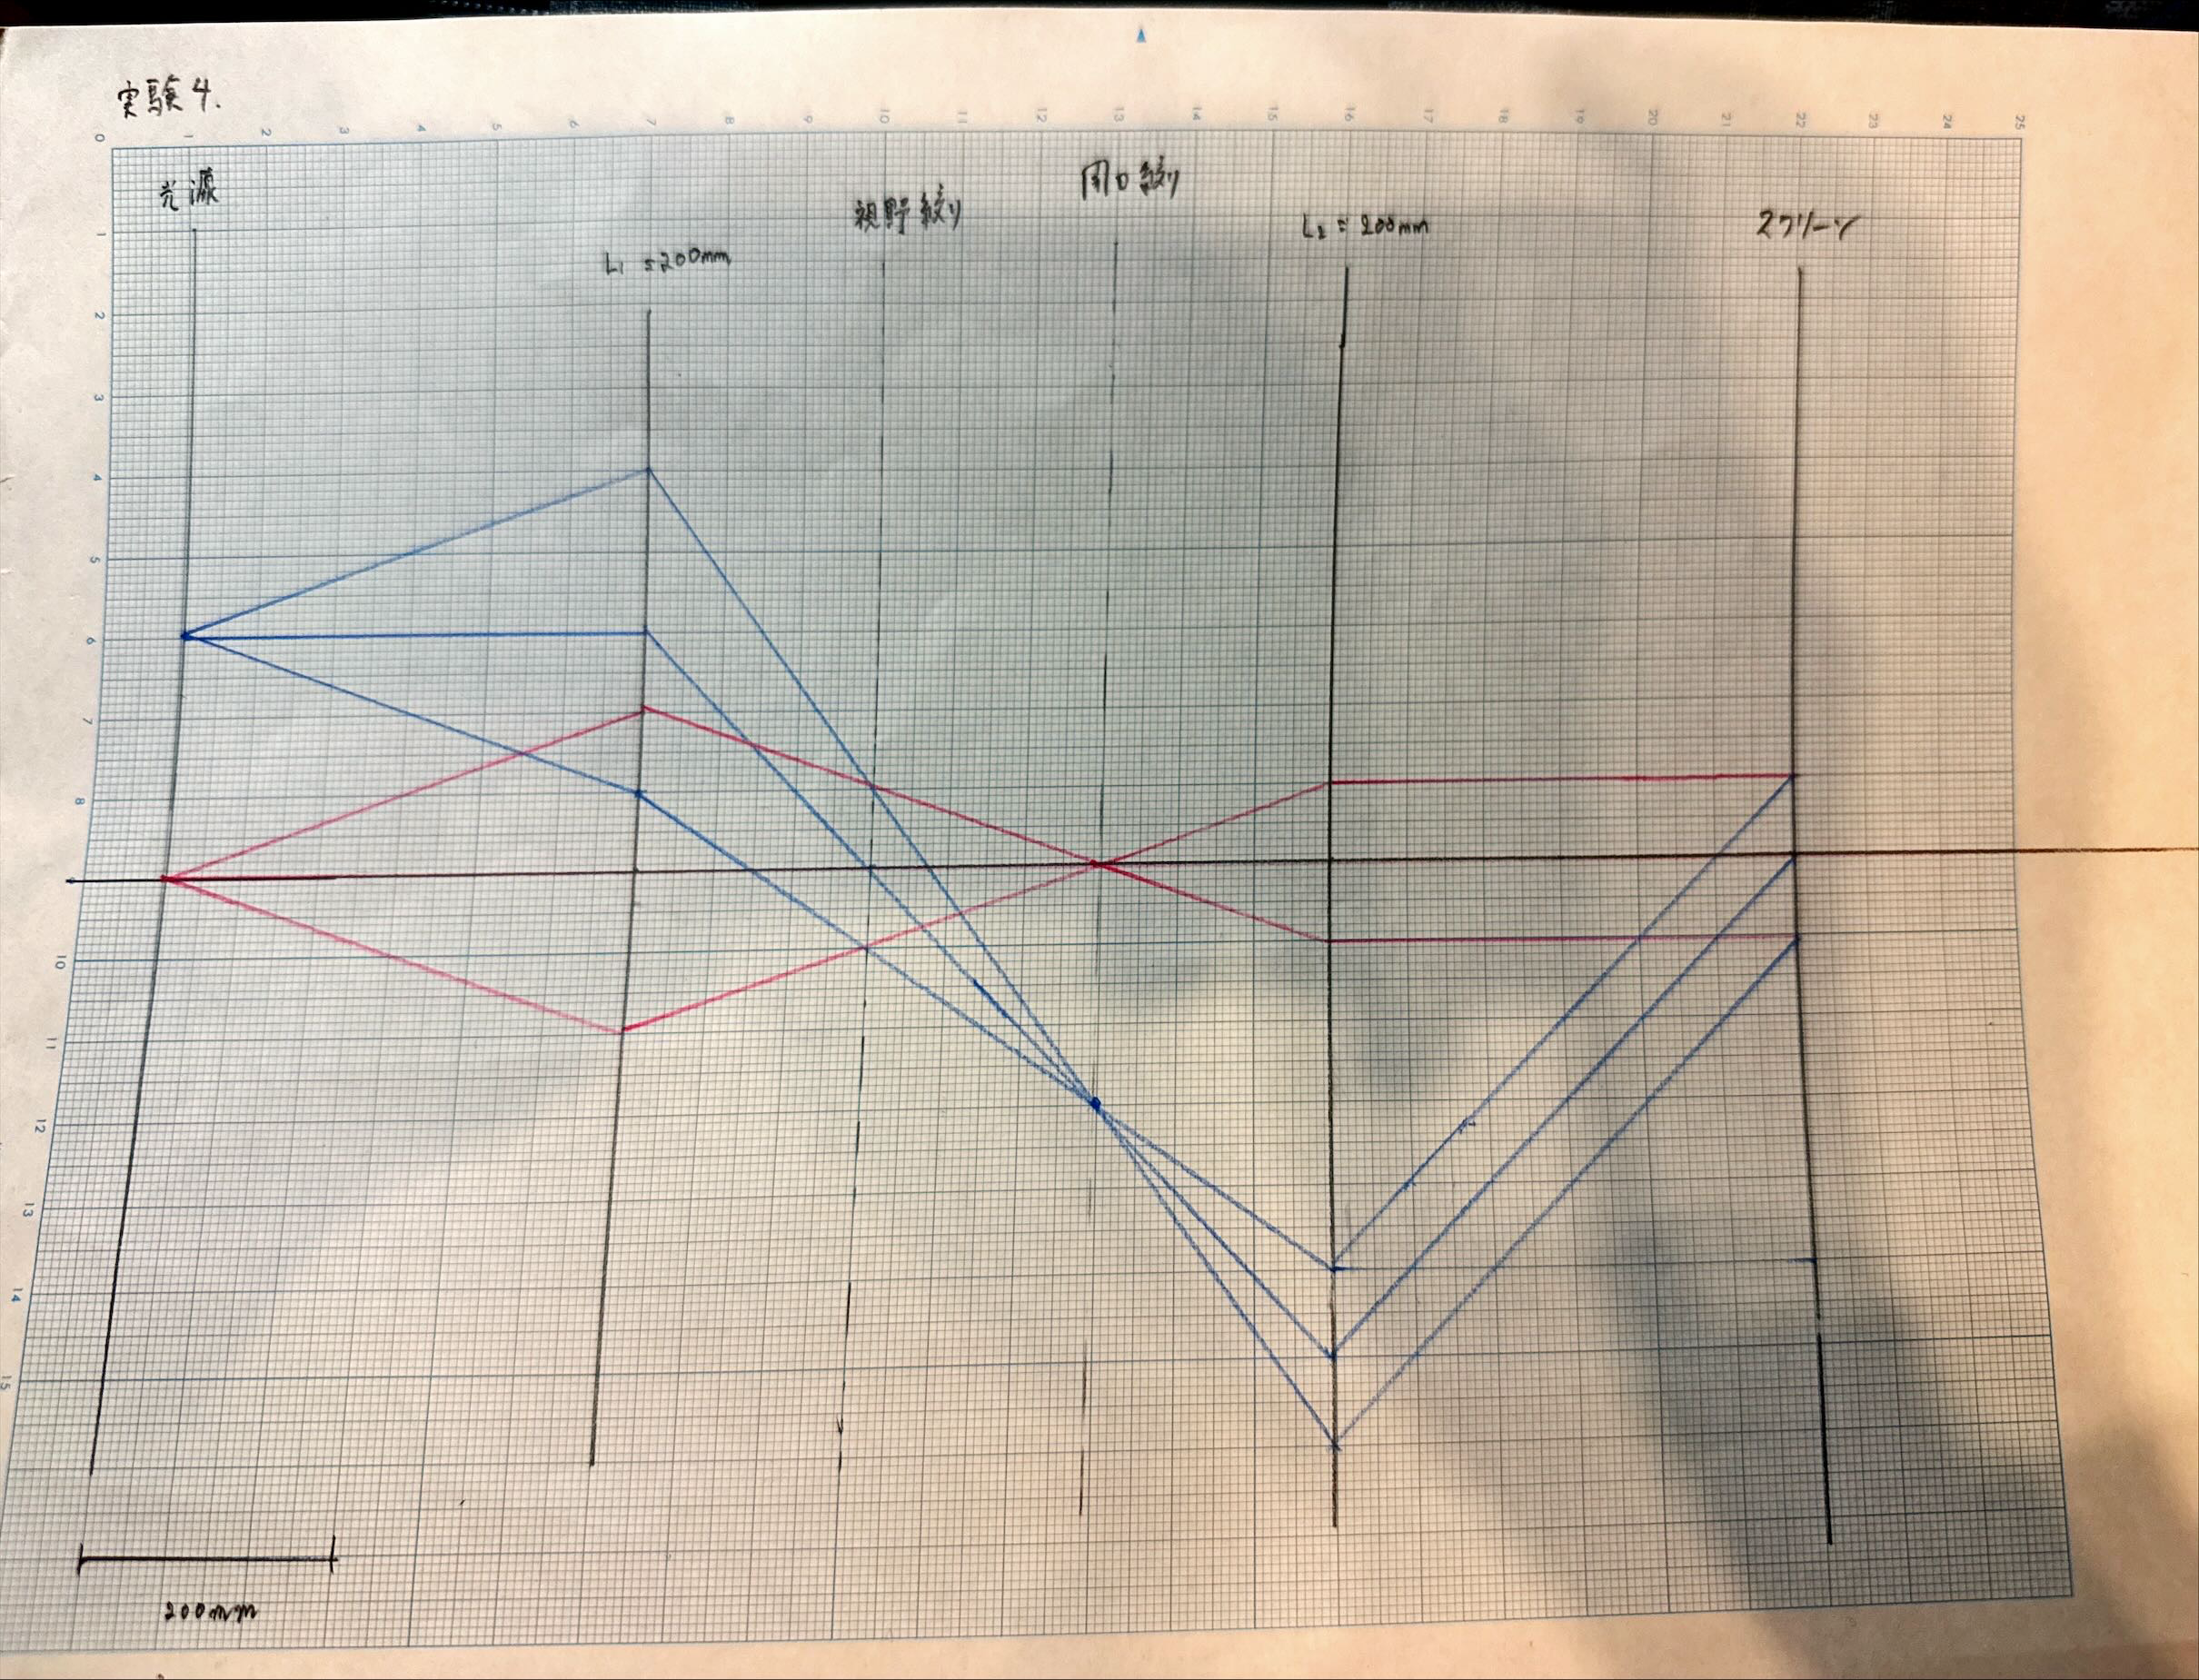
\includegraphics[width=0.98\linewidth]{./figure/4_sakuzu.png}
  \caption{実験4で作成したケーラー照明の作図。視野絞りが試料面に結像し、光源像が開口絞り面に結像することがわかる。}
  \label{fig:kohler_sakuzu}
\end{figure}


\subsection*{\underline{結果}}
視野絞りが試料面に、光源像が開口絞り面にそれぞれ結像していることを確認し、
両絞りを独立に調整することで視野の一様性と照明の角度分布(NA)を独立に制御できることが確認された。

  \subsection*{\underline{考察}}
  \subsection*{レポートのための課題4}

  \begin{enumerate}
    \item 視野絞り:コンデンサーレンズに関して、スクリーンと共役な位置にあるから。\\
開口絞り:集光レンズに関して、光源と共役な位置にあるから。
    \item 図\ref{fig:kohler_sakuzu}にあるように、800mmの位置はコンデンサーレンズの焦点であるが、同時に光源の集光レンズに関する共役点でもある。
    これによって、開口絞りの位置に光源があるのと同様の状態が実現しており、一様な照明が実現する。
  \end{enumerate}

\section*{実験5. 顕微鏡の組立}
\subsection*{\underline{目的}}
実験4で構成したケーラー照明系を照明系として用い、対物レンズ($f=70\,\mathrm{mm}$)と結像レンズ($f=500\,\mathrm{mm}$)からなる観察系を組み上げて、簡易顕微鏡を構成することを目的とする。
その上で、格子縞試料($20\,\mu\mathrm{m}$、$100\,\mu\mathrm{m}$間隔)の像がカメラ上に結像することを確認し、必要な焦点調整と光軸調整を行う。
さらに、視野絞り直後に650\,nmフィルタや450\,nmフィルタを挿入した際の像の変化を観察する。

\subsection*{\underline{方法}}
実験4で調整したケーラー照明系を維持したまま、試料位置に格子縞試料(それぞれ25\,$\mu\mathrm{m}$, 100\,$\mu\mathrm{m}$)を設置した。
次に、試料の直後に対物レンズ(焦点距離 $f=70\,\mathrm{mm}$)を光軸上に配置し、
対物レンズによって得られる中間像を結像レンズ(焦点距離 $f=500\,\mathrm{mm}$)でカメラ撮像面に結像させる観察系を構成した。

\begin{figure}[H]
  \centering
  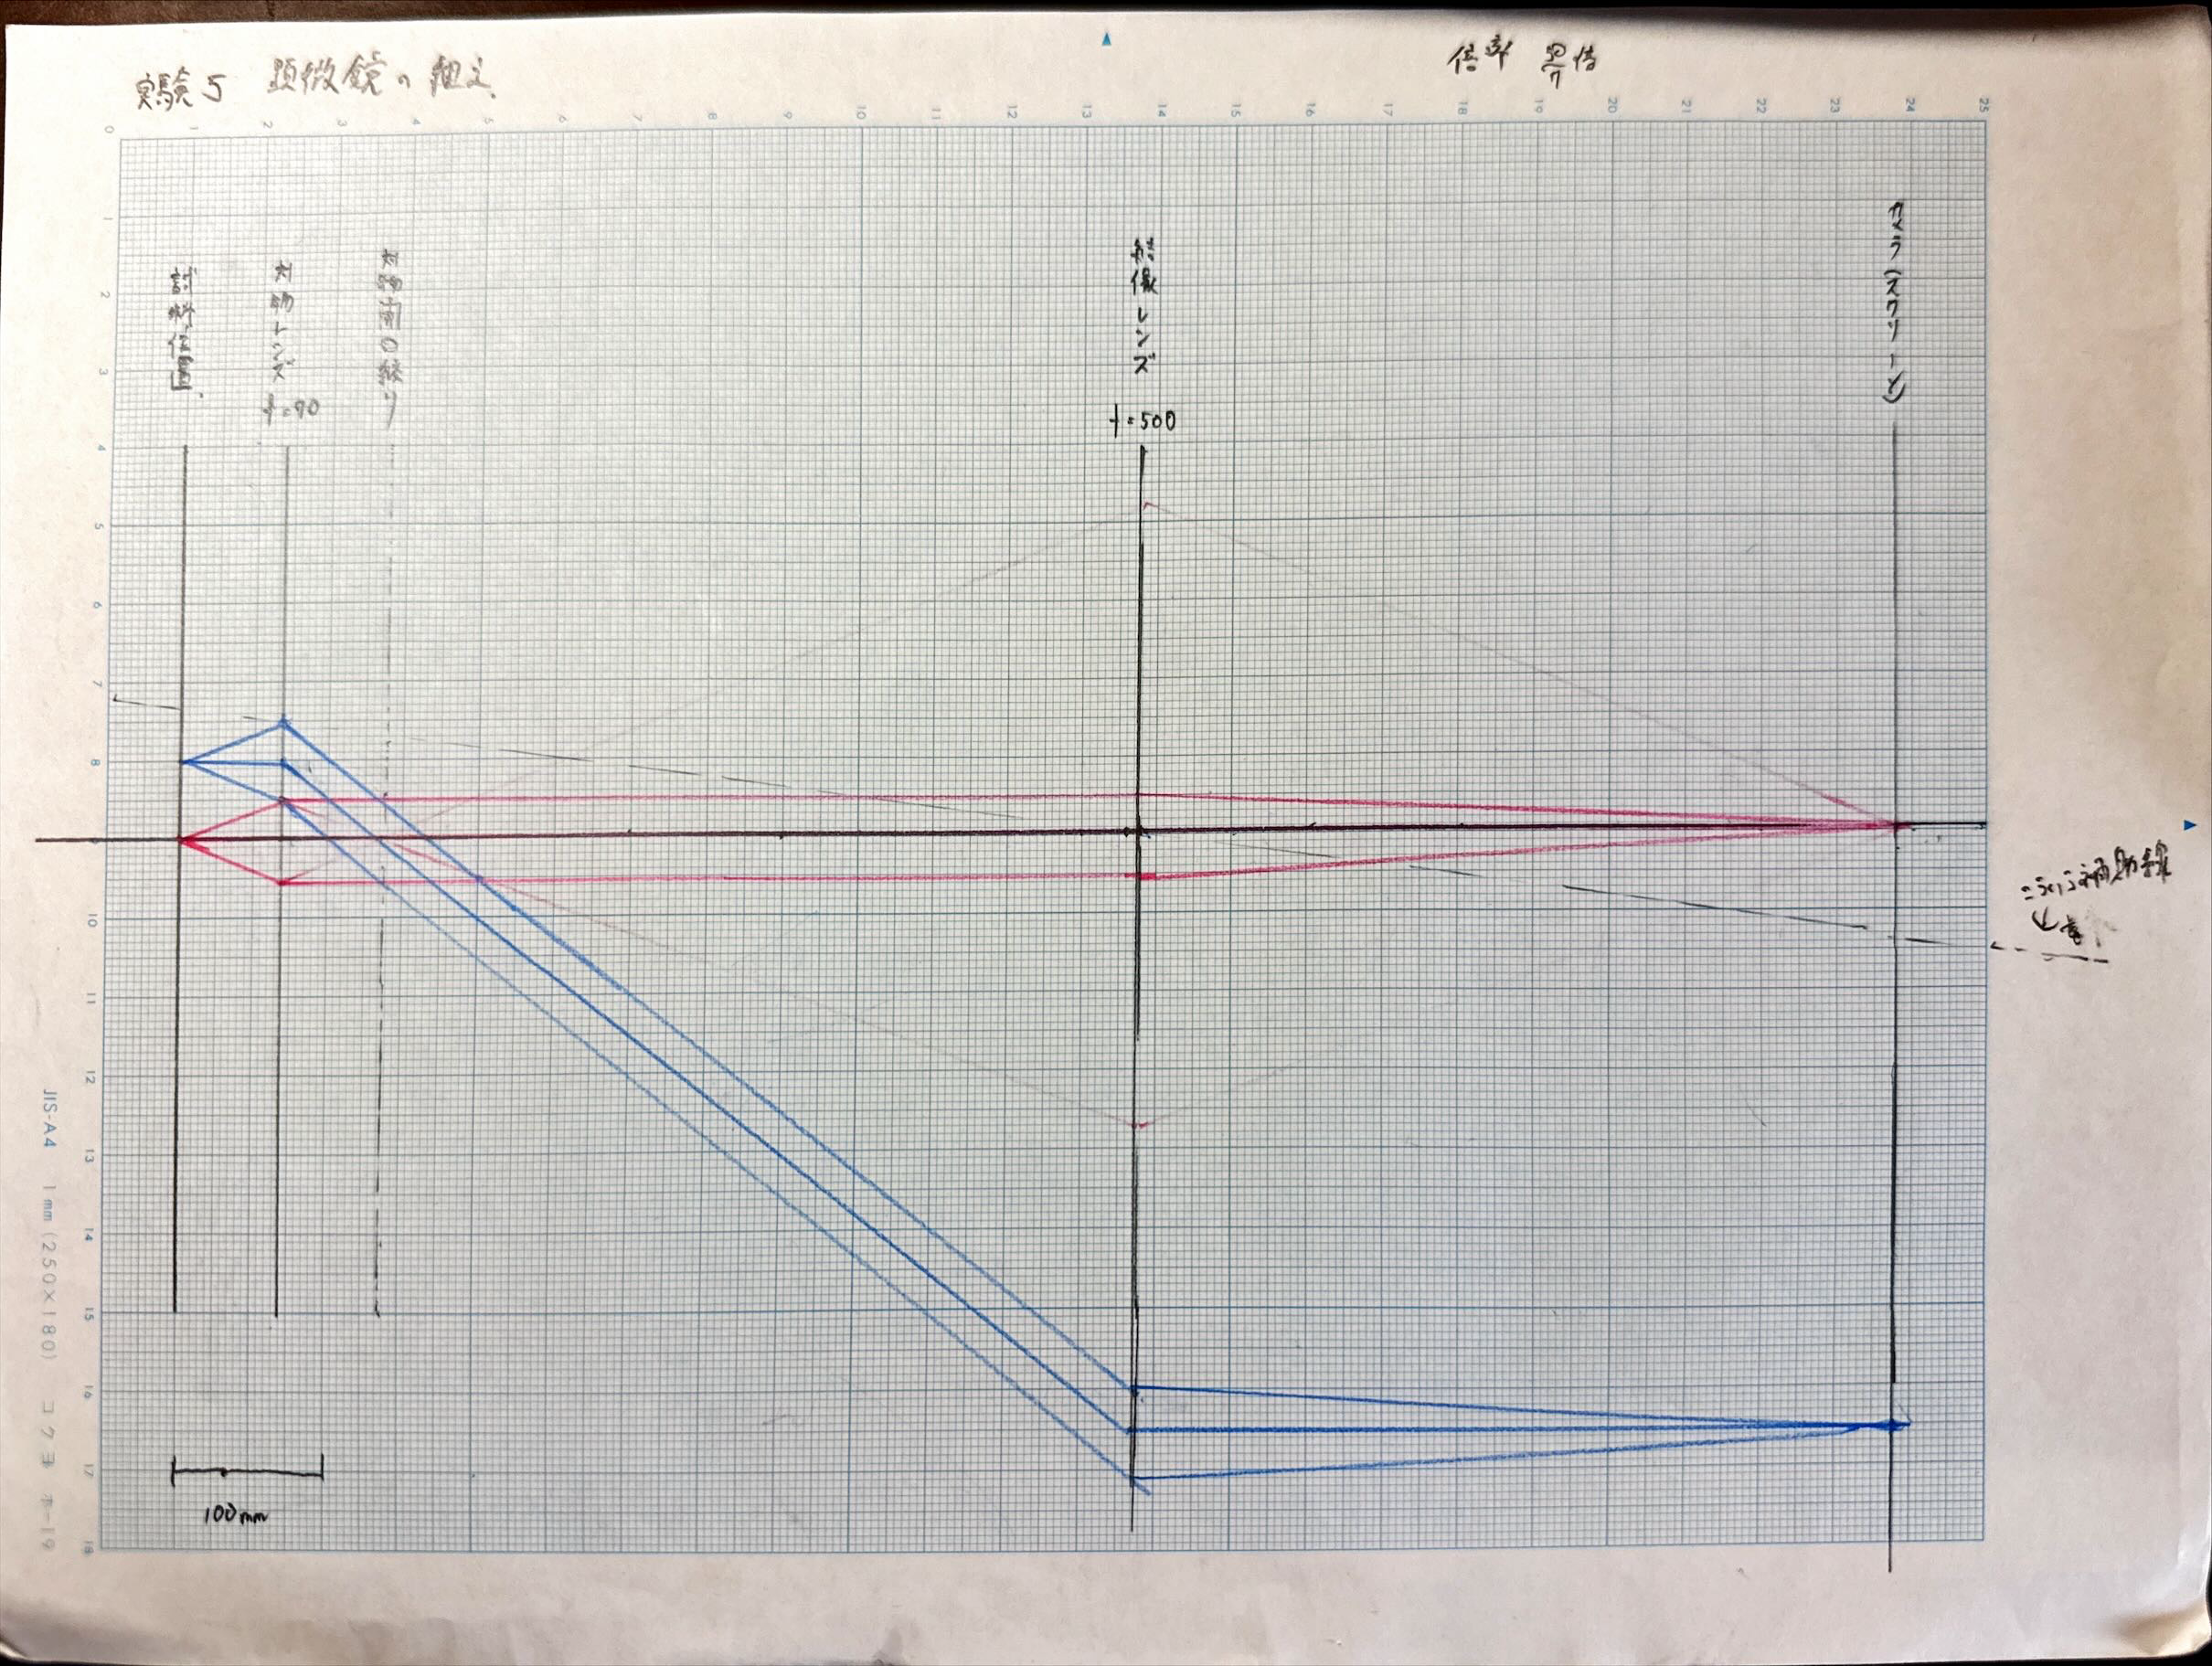
\includegraphics[width=0.95\linewidth]{./figure/5_micro.png}
  \caption{顕微鏡光学系の作図。ケーラー照明系を照明系として用い、対物レンズと結像レンズからなる観察系を組み上げた。}
  \label{fig:microscope_setup}
\end{figure}

光軸調整は、(i)各レンズ・絞りの中心が同一直線上に来るようにレール上の高さと横位置を合わせ、
(ii)カメラ画像上で像のケラレや片ボケが最小となるようにレンズ角度と位置を微調整することで行った。
焦点調整は、カメラを結像レンズ後方で前後に移動させ、格子縞のコントラストが最大となる位置を探すことで行った。

格子縞試料として、周期 $20\,\mu\mathrm{m}$ および $100\,\mu\mathrm{m}$ の2種類を用い、それぞれについて同様に結像を確認し、必要に応じて試料位置および対物レンズ位置を微調整した。

また、視野絞り直後に中心波長 650\,nm および 450\,nm のバンドパスフィルタを挿入し、
フィルタなしの場合と比較して、像の明るさ、コントラスト、分解能(縞の見え方)の変化を観察・記録した。

\clearpage
\subsection*{\underline{結果}}

本実験では、格子縞試料($20\,\mu\mathrm{m}$、$100\,\mu\mathrm{m}$)を用いて顕微鏡像を撮影し、カラーフィルタおよび各絞りの開閉が像に与える影響を比較した。

\subsubsection*{格子縞像の結像確認(フィルタなし)}
まず、$100\,\mu\mathrm{m}$ 間隔の格子縞試料を試料ホルダに固定し、カメラ上に格子縞像が結像することを確認した後、その像を撮影した(図\ref{fig:exp5_100um_nofilter})。
次に、$20\,\mu\mathrm{m}$ 間隔の格子縞試料に戻し、同様に焦点および光軸を微調整して像を得た。

\begin{figure}[H]
  \centering
  \includegraphics[width=0.95\linewidth]{./figure/20um.png}
  \includegraphics[width=0.95\linewidth]{./figure/5_100um_nofilter.png}
  \caption{$20\,\mu\mathrm{m}$,$100\,\mu\mathrm{m}$ 格子縞試料の顕微鏡像(フィルタなし)。まず像がカメラ上に結像することを確認した後に撮影した。}
  \label{fig:exp5_100um_nofilter}
\end{figure}

\subsubsection*{650\,nmフィルタ挿入時($20\,\mu\mathrm{m}$)}
視野絞り直後に中心波長 650\,nm のフィルタを挿入すると、像は暗くなり、初期状態ではピントが外れて見えた。
そこで試料位置を微調整し、$20\,\mu\mathrm{m}$ 格子縞像が再び明瞭に観察される条件を探索して撮影した(図\ref{fig:exp5_20um_650})。

\begin{figure}[H]
  \centering
  \includegraphics[width=0.95\linewidth]{./figure/650nm_20um_defocus.png}
  \includegraphics[width=0.95\linewidth]{./figure/650nm_20um_focus.png}
  \caption{$20\,\mu\mathrm{m}$ 格子縞試料の顕微鏡像(650\,nmフィルタ挿入)。フィルタ挿入後に試料位置を再調整して撮影した。}
  \label{fig:exp5_20um_650}
\end{figure}

\subsubsection*{450\,nmフィルタ挿入時($20\,\mu\mathrm{m}$)}
次にフィルタを中心波長 450\,nm に変更した。
再び像がぼける傾向が見られたため、試料位置を再調整し、$20\,\mu\mathrm{m}$ 格子縞像を撮影した(図\ref{fig:exp5_20um_450})。

\begin{figure}[H]
  \centering
  \includegraphics[width=0.95\linewidth]{./figure/450nm_20um_defocus.png}
  \includegraphics[width=0.95\linewidth]{./figure/450nm_20um_focus.png}
  \caption{$20\,\mu\mathrm{m}$ 格子縞試料の顕微鏡像(450\,nmフィルタ挿入)。フィルタ変更後に試料位置を再調整して撮影した。}
  \label{fig:exp5_20um_450}
\end{figure}

\subsubsection*{$20\,\mu\mathrm{m}$および$100\,\mu\mathrm{m}$格子縞像(450\,nm)}
450\,nmフィルタを挿入した状態のまま、試料位置を調整して $20\,\mu\mathrm{m}$ および $100\,\mu\mathrm{m}$ 格子縞の両方について像を撮影した(図\ref{fig:exp5_20um_450_final}, 図\ref{fig:exp5_100um_450_final})。

\begin{figure}[H]
  \centering
  \includegraphics[width=0.95\linewidth]{./figure/450nm_20um_focus.png}
  \caption{$20\,\mu\mathrm{m}$ 格子縞試料の顕微鏡像(450\,nmフィルタ、最終調整後)。}
  \label{fig:exp5_20um_450_final}
\end{figure}

\begin{figure}[H]
  \centering
  \includegraphics[width=0.95\linewidth]{./figure/450nm_100um.png}
  \caption{$100\,\mu\mathrm{m}$ 格子縞試料の顕微鏡像(450\,nmフィルタ、最終調整後)。}
  \label{fig:exp5_100um_450_final}
\end{figure}

\subsubsection*{絞り開閉による像変化}
最後に、照明側の視野絞りおよび開口絞り(コンデンサ絞り)、ならびに観察側の開口絞り(対物絞り)をそれぞれ開閉し、カメラに写る像の変化を観察して撮影した。
代表例として、視野絞りの開閉(図\ref{fig:exp5_field_stop})、照明開口絞りの開閉(図\ref{fig:exp5_illum_aperture})、対物絞りの開閉(図\ref{fig:exp5_obj_aperture})の結果を示す。

\begin{figure}[H]
  \centering
  \includegraphics[width=0.95\linewidth]{./figure/450nm_20um_siya.png}
  \caption{視野絞りの開閉による像の変化(代表例)。照明される領域(視野)が変化する。}
  \label{fig:exp5_field_stop}
\end{figure}

\begin{figure}[H]
  \centering
  \includegraphics[width=0.95\linewidth]{./figure/450nm_20um_Csibori.png}
  \caption{照明側開口絞り(コンデンサ絞り)の開閉による像の変化(代表例)。照明の角度分布(NA)が変化する。}
  \label{fig:exp5_illum_aperture}
\end{figure}

\begin{figure}[H]
  \centering
  \includegraphics[width=0.95\linewidth]{./figure/450nm_20um_Taibutusibori.png}
  \caption{観察側開口絞り(対物絞り)の開閉による像の変化(代表例)。像の明るさ、コントラスト等が変化する。}
  \label{fig:exp5_obj_aperture}
\end{figure}

\clearpage

\subsection*{\underline{考察}}
\subsection*{レポートのための課題5}
\begin{enumerate}
  \item \textbf{カラーフィルタ挿入時に観察された現象。}\\
  650\,nm、450\,nm のバンドパスフィルタを視野絞り直後に挿入すると、像がぼやけ、いったんピントが外れたように見えた。
  これは、レンズの色収差により焦点位置が波長依存でわずかに変化することによると解釈できる。

  \item \textbf{ImageJによる倍率の算出と作図結果との比較。}\\
  撮影像(例:図\ref{fig:exp5_20um_450_final}、図\ref{fig:exp5_100um_450_final})を ImageJ で開き、格子縞の周期に相当する距離を画素単位で測定した。
  既知の試料周期 $p$($20\,\mu\mathrm{m}$ または $100\,\mu\mathrm{m}$)に対して、画像上の周期を $p_{\mathrm{img}}$ とすると、倍率は
  \[
    M_{\mathrm{meas}}=\frac{p_{\mathrm{img}}}{p}
  \]
  で与えられる。
  一方、本顕微鏡は、試料を対物レンズの前側焦点($f_{\mathrm{obj}}=70\,\mathrm{mm}$)付近に置き、対物で平行光を作って結像レンズ($f_{\mathrm{tube}}=500\,\mathrm{mm}$)でカメラ面に結像させる無限遠補正型の配置である(図\ref{fig:microscope_setup})。
  このとき理論倍率は
  \[
    M_{\mathrm{th}}=\frac{f_{\mathrm{tube}}}{f_{\mathrm{obj}}}=\frac{500}{70}\simeq 7.14
  \]
  で見積もられる。
  ImageJ から得た倍率 $M_{\mathrm{meas}}=7.27$ は $M_{\mathrm{th}}$ と同程度であり、作図に基づく倍率見積もりと整合した。

  \item \textbf{各絞りの開閉による像変化。}\\
  視野絞りを閉じると、試料面に結像する絞り像が縮小するため、照明される領域(視野)が狭くなり、不要な周辺光が減って迷光が抑制された(図\ref{fig:exp5_field_stop})。
  照明側の開口絞り(コンデンサ絞り)を閉じると、試料に入射する角度分布(照明NA)が小さくなり、一般にコントラストは増す一方で分解能は低下し、像は暗くなる傾向を示した(図\ref{fig:exp5_illum_aperture})。
  観察側の開口絞り(対物絞り)を閉じると、像形成に寄与する光線(観察NA)が制限され、像は暗くなり、細部(格子縞のエッジ)の再現性が低下する一方で、見かけのコントラストが変化した(図\ref{fig:exp5_obj_aperture})。
\end{enumerate}

\section*{実験6. フーリエ変換と空間周波数フィルタリング}
% \subsection*{目的}
% 本実験の目的は、レンズによって実現されるフーリエ変換を光学系として具体的に観察し、像の空間周波数成分がどのように分布するかを理解することである。
% さらに、フーリエ面に空間フィルタ(遮蔽板や開口)を挿入して低周波・高周波成分を選択的に通過/遮断し、像のぼけ、エッジ強調、周期構造の抽出などの変化を確認する。
% これらを通じて、回折とフーリエ変換の対応関係、および顕微鏡像形成における空間周波数フィルタリングの基本概念を習得する。

% \subsection*{方法}
% 本実験では強度の高い光をカメラに入射させるため、手順を確認しつつ露光時間を短く設定して測定を行った。
% まず顕微鏡を通常の結像配置とし、格子縞試料の像がカメラ上に得られることを確認した。
% 次に、コンデンサー絞りをできるだけ絞り、カメラの露光時間を 1\,ms 以下に設定した上で、対物絞りを取り外した。
% その後、カメラを対物絞り位置(フーリエ面)に移動し、前後位置を微調整して格子縞の回折像(フーリエ像)が最も鮮明となる条件を探索した。
% この条件で、$20\,\mu\mathrm{m}$ および $100\,\mu\mathrm{m}$ 間隔の格子縞試料について回折像を撮影した。

% 続いてカメラを元の像面位置に戻し、コンデンサー絞りと露光時間を調整して試料像が再び得られることを確認した。
% 最後に、対物絞り位置に空間フィルタ(縦スリット、横スリットを含む)を挿入し、通過させる空間周波数成分を変化させながら、像がどのように変化するかを観察して撮影した。

\textcolor{red}{\textbf{ちょっと内容がムズかしかったので、一旦保留で!}}

\clearpage

\section*{実験7. 振幅コントラストと位相コントラスト}
\subsection*{\underline{目的}}
本実験の目的は、これまで用いてきた白黒コントラストが明瞭な試料と、位相物体である哺乳類細胞(HeLa cell)とを比較することで、
顕微鏡像における振幅コントラストおよび位相コントラストの生成機構を理解することである。

\subsection*{\underline{方法}}
まず、これまで用いていた白黒コントラストが明瞭な試料を用い、カメラ位置を調整して像が鮮明に観察できる状態に合わせた。
次に、試料を哺乳類細胞(HeLa cell)に交換し、同一の光学条件で細胞像を撮影した。
その後、初期条件からカメラ位置を光軸方向に前後させた場合の像変化を観察し、それぞれの条件で細胞像を撮影した。
さらに、コンデンサ絞りを閉じた場合についても像変化を観察し、それぞれの条件で細胞像を撮影した。

\clearpage
\onecolumn

\subsection*{\underline{結果}}
HeLa 細胞について、(i) 焦点を合わせた基準条件、
(ii) カメラ位置を光軸方向に前後させた条件、
(iii) コンデンサ絞りを閉じた条件の3通りで撮影を行った。
以下に、それぞれの条件で得られた細胞像を示す。

\begin{figure}[H]
  \centering
  \includegraphics[width=0.9\linewidth]{./figure/hela.png}
  \caption{HeLa細胞の明視野像。白黒コントラストが明瞭な試料で調整した光学条件を保ったまま、カメラ位置を焦点に合わせて撮影した。位相物体である細胞は透過強度差が小さく、輪郭のコントラストは弱い。}
  \label{fig:exp7_default}
\end{figure}

\begin{figure}[H]
  \centering
  \includegraphics[width=0.48\linewidth]{./figure/hela_close_1cm.png}
  \includegraphics[width=0.48\linewidth]{./figure/hela_far_1cm.png}
  \caption{HeLa細胞像。基準条件からカメラ位置を光軸方向に前後へ 1\,cm 移動させて撮影した(デフォーカス条件)。左が1cm近づけた写真で、右が1cm遠ざけた写真である。位相差が強度差へ変換され、細胞輪郭が陰影として可視化された。前後移動により陰影の向きがおよそ反転している様子も確認できる。}
  \label{fig:exp7_defocus}
\end{figure}

\begin{figure}[H]
  \centering
  \includegraphics[width=0.48\linewidth]{./figure/hela_sibori.png}
  \includegraphics[width=0.48\linewidth]{./figure/hela_sibori_close_1cm.png}
  \caption{HeLa細胞像。コンデンサ絞りを閉じた条件で撮影した像。照明NAの低下により位相差由来のコントラストが増大し、細胞輪郭が明瞭に観察された。さらにデフォーカスを与えることで、輪郭強調が顕著となった。}
  \label{fig:exp7_aperture}
\end{figure}

\twocolumn

\subsection*{\underline{考察}}

\subsection*{レポートのための課題7}

HeLa 細胞像が見えやすくなった理由を、(A)カメラ位置の前後移動(デフォーカス)による効果と、
(B)コンデンサ絞りを閉じることによる効果と分けて考察する。以下にそれぞれの要因を整理する。

\subsubsection*{(A) カメラ位置の前後移動(デフォーカス)}
\begin{enumerate}
  \item \textbf{位相差が強度差へ変換されたこと(位相コントラストの生成)。}\\
  HeLa 細胞は吸収が小さく、主に屈折率や厚みの違いによって位相のみを変化させる位相物体である。
  焦点を厳密に合わせた明視野条件では、透過光の強度差が小さいためコントラストが弱い。
  一方、カメラ位置を前後に移動させると、位相の空間変調が回折を通じて振幅変調へと変換され、
  細胞輪郭が明暗(陰影)として可視化される。

  \item \textbf{前後移動で陰影の向きが変化すること。}\\
  デフォーカスの符号(像面が焦点面の前後どちらにあるか)を変えると、位相から強度への変換の符号が変化し、
  輪郭に現れる明暗の向きが反転する。
  図\ref{fig:exp7_defocus}で観察された陰影の向きの変化は、この性質と整合的である。
\end{enumerate}

\subsubsection*{(B) コンデンサ絞りを閉じる}
\begin{enumerate}
  \item \textbf{照明NAの低下による位相由来コントラストの増大。}\\
  コンデンサ絞りを閉じると、試料に入射する光の角度分布が狭くなり、照明の開口数(NA)が低下する。
  これにより、異なる方向からの光の重ね合わせが減少し、位相差による干渉効果が平均化されにくくなる。
  その結果、位相差由来のコントラストが増大し、細胞像が見えやすくなる。

  \item \textbf{空間コヒーレンスの向上。}\\
  照明の角度分布が狭くなると、試料面での空間コヒーレンスが向上する。
  空間コヒーレンスが高い条件では、位相差による干渉効果が顕著となり、位相物体の構造が強度分布として観察されやすくなる。

  \item \textbf{近軸近似に近づくことによる像形成の単純化。}\\
  照明NAを下げることは、主に光軸近傍を通る光線のみを用いることに対応する。
  このとき光学系は近軸近似がより良く成り立つ条件となり、位相変化が単純な光路差として像形成に反映されやすくなる。
  \[
  \sin\theta \simeq \theta \simeq \tan\theta
  \]
\end{enumerate}


コントラストと分解能はトレードオフだと言える。コンデンサ絞りを閉じた条件では、位相由来のコントラストは増大する一方で、高角度成分が除去されるため分解能は低下し、像は暗くなる傾向を示す。
本実験では、分解能低下よりもコントラスト向上の効果が支配的であったため、細胞輪郭が見えやすくなったと解釈できる。

\clearpage
\section*{実験8. 生物試料の観察}
\subsection*{\underline{目的}}
アナカリスの原形質流動およびクラミドモナスの遊泳運動を動画撮影し、生物試料の運動を定性的・定量的に観察する。

\subsection*{\underline{方法}}
生物試料としてアナカリス(オオカナダモ)およびクラミドモナス(コナミドリムシ)を作成した顕微鏡で観察し、それぞれについて動画撮影を行った。
まず、開口絞りが十分に開いていることを確認し、撮影時のフレームレート(撮影速度)を記録した。
次に、アナカリスでは細胞内の顆粒の移動を指標として原形質流動の様子を動画撮影した。
続いて、クラミドモナスでは視野内を移動する個体の運動を動画撮影し、遊泳していない場合には沈降する様子を撮影した。

\subsection*{\underline{結果}}
アナカリスおよびクラミドモナスについて動画撮影を行い、代表フレームを静止画として図に示す。
撮影時のフレームレートは アナカリスは$1\,\mathrm{fps}$、クラミドモナスは$10\,\mathrm{fps}$であった。

\subsubsection*{アナカリス(原形質流動)}
アナカリス細胞内の顆粒が一定方向に移動する様子が観察された。
代表フレームを図\ref{fig:exp8_anacharis}に示す。

\begin{figure}[H]
  \centering
  \includegraphics[width=0.95\linewidth]{./figure/exp8_anacharis_frame.png}
  \caption{アナカリスの原形質流動の代表フレーム。動画中で細胞内顆粒が一定方向に移動する様子が確認された。}
  \label{fig:exp8_anacharis}
\end{figure}

\subsubsection*{クラミドモナス(遊泳運動)}
クラミドモナスが視野内を移動する様子を観察した。
代表フレームを図\ref{fig:exp8_chlamy}に示す。
(遊泳が見られない個体については、沈降する様子を記録した。)

\begin{figure}[H]
  \centering
  \includegraphics[width=0.95\linewidth]{./figure/exp8_chlamy_frame.png}
  \caption{クラミドモナスの運動の代表フレーム。動画中で個体が視野内を移動する様子を記録した。}
  \label{fig:exp8_chlamy}
\end{figure}

\textcolor{red}{Q.これ、どう見せればいいの? 動画を静止画にして伝えるの難しい。}

\subsection*{\underline{考察}}
\subsection*{レポートのための課題8}

本実験では、クラミドモナスの遊泳運動を観察し、その遊泳速度を求めることを目的とした。
しかし、本班で観察したクラミドモナスは活性が低く、明瞭な遊泳運動が確認できなかった。
そこで TA の判断のもと、他班が撮影した動画データを用いて解析を行った。

動画のフレームレートを $10\,\mathrm{fps}$ とし、
連続する 10 フレーム間(時間 $\Delta t = 10/f_{\mathrm{fps}}$)におけるクラミドモナスの移動距離 $\Delta x$ を測定した。
各区間について速度
\[
v = \frac{\Delta x}{\Delta t}
\]
を求め、その平均値をクラミドモナスの遊泳速度とした。

測定結果を表\ref{tab:exp8_velocity}に示す。

\onecolumn

\begin{table}[H]
\centering
\caption{クラミドモナスの遊泳距離および速度(10フレーム間)}
\label{tab:exp8_velocity}
\begin{tabular}{cccc}
\toprule
測定番号 & 移動距離 $\Delta x$ [$\mathrm{px}$] & 時間 $\Delta t$ [s] & 速度 $v$ [$\mu\mathrm{m/s}$] \\
\midrule
1 & 180.27 & 1.0 & 128.94 \\
2 & 219.32 & 1.0 & 156.87 \\
3 & 160.46 & 1.0 & 114.77 \\
4 & 222.99 & 1.0 & 159.50 \\
\midrule
平均 &  & & $\bar v= 140\,\mu\mathrm{m/s}$ \\
\bottomrule
\end{tabular}
\end{table}

\twocolumn

以上より、クラミドモナスの遊泳速度は
\[
\bar v = 140\,\mu\mathrm{m/s}
\]
と見積もられた。

\section*{実験9. 暗視野照明と限外顕微鏡}
\subsection*{\underline{目的}}
暗視野照明を構成して回折限界以下(200\,nm)の金ナノ粒子を輝点として観察し、
絞り条件およびレンズの有効径が像の明るさと大きさに与える影響を確認する。

\subsection*{\underline{方法}}
まず、$500\,\mu\mathrm{m}$ 格子縞試料を用い、格子縞の中心線がカメラ画像の中央に一致するように試料位置を調整した。
次に、カメラの蓋を閉めて受光面に外光が入らないようにし、以降は試料ホルダより下流の光学素子は動かさない条件で調整を行った。

照明側のレンズを取り外し、コンデンサレンズとして焦点距離 $f=70\,\mathrm{mm}$ のレンズを試料から $70\,\mathrm{mm}$ の位置に配置した。
ミラーを平行移動させてレーザー光がコンデンサレンズに入射するように調整し、ミラーで反射させたレーザー光が入射光と平行に進むことを確認した。
続いて、コンデンサレンズ位置を微調整して格子縞の中心にレーザー光が当たるように合わせた。
対物開口絞りを適度に閉じ、レーザーの直達光が対物レンズに入射しない条件を作ったうえで、試料で散乱された光のみが対物レンズを通過してカメラに結像する暗視野照明であることを確認した。

試料を金ナノ粒子(粒径 $200\,\mathrm{nm}$)に交換し、回折限界以下の粒子が輝点として観察できることを確認して撮影した。
さらに、絞りの直径を $5\text{--}10\,\mathrm{mm}$ 程度に設定し、複数(5個程度)の粒子について像を撮影した。
得られたコロイド像から輝点像の大きさを測定し、絞り条件(レンズの有効径)との関係を理論値と比較した。

\subsection*{\underline{結果}}
暗視野照明の条件(直達光が対物レンズに入射せず、散乱光のみが結像する条件)を実現し、
金ナノ粒子(粒径 $200\,\mathrm{nm}$)が輝点として観察できることを確認した。
代表的なコロイド像を図\ref{fig:exp9_overview}に示す。

\begin{figure}[H]
  \centering
  \includegraphics[width=0.95\linewidth]{./figure/exp9_overview.png}
  \caption{暗視野照明下で観察した金ナノ粒子($200\,\mathrm{nm}$)のコロイド像(代表例)。粒子は背景に対して輝点として観察される。}
  \label{fig:exp9_overview}
\end{figure}

絞り直径を $5\text{--}10\,\mathrm{mm}$ の範囲で変化させて複数粒子を撮影し、輝点像の見かけの大きさを測定した。
定量結果の整理(絞り直径と輝点像径の関係)は考察(課題9)に示す。


% --- 実験9 考察・課題9 ここから挿入 ---
\subsection*{\underline{考察}}
\subsection*{レポートのための課題9(考察)}

本実験10では、観察中の絞り直径は常に $D=10\,\mathrm{mm}$ に固定していた。
実験2で得られた回折理論に基づけば、有効径 $D=10\,\mathrm{mm}$ に対する集光像の大きさは
\[
d_{\mathrm{th}} \simeq 38\,\mu\mathrm{m}
\]
と見積もられる。

一方、暗視野照明下で観察した金ナノ粒子の輝点像について、
ガウスフィッティングにより得られた幅パラメータは
$d = 2.35,\,2.61,\,2.46,\,2.95\,\mathrm{px}$ であった。
ここでカメラの画素サイズ $1\,\mathrm{px}=5.2\,\mu\mathrm{m}$ を用いると、
対応する像の大きさは
\[
d \simeq 12\text{--}15\,\mu\mathrm{m}
\]
となる。

この測定値は、回折理論から見積もられる $d_{\mathrm{th}} \simeq 38\,\mu\mathrm{m}$ よりも十分に小さく、
本実験で観察された輝点像が、対物レンズの有効径による分解能限界を超えて
「小さく見えている」ことを示している。

これは、暗視野照明および限外顕微鏡では粒子の形状を分解して観察しているのではなく、
粒子による散乱光の存在を輝点として検出しているためである。
すなわち、本実験結果は、回折限界以下の粒子であっても、
散乱光を用いればその存在を検出できることを示している。

% --- 実験9 考察・課題9 ここまで ---

% \subsubsection*{Day1}
% 目に見えるのが嬉しい。
\end{document}

% 5の結果とレポートのための課題5めっちゃ適当。chatGPTが書いてる。後で要修正
% 実験4までDONE
% NA: 実験5。目的の文章だいぶ怪しい。

platex main.tex
dvipdfmx main.dvi